\chapter{O przestrzeni rozwiązań}
W rozdziale przedstawiono definicje przestrzeni rozwiązań oraz sieci optimów lokalnych.
Opisane zostały również miary analizowane w pozostałej części pracy, oraz operacja 2-exchange stanowiąca operator permutacji w wykorzystanych algorytmach próbkowania.

Przestrzeń rozwiązań (Krajobraz adaptacyjny, ang. Fitness Landscape) jest pojęciem wywodzącym się z biologii ewolucyjnej.
W kontekście biologicznym jest to model opisujący relację między genotypem i fenotypem organizmów, a ich przystosowaniem (ang. fitness),
które jest miarą opisującą sukces reprodukcyjny \cite{FRAGATA201969}.

W kontekście optymalizacji Fitness landscape to trójka $(S, V, f)$, gdzie:
\begin{itemize}
      \item $S$ jest zbiorem wszystkich możliwych rozwiązań - przestrzenią przeszukiwania,
      \item $V$ jest funkcją przypisującą każdemu rozwiązaniu $s\in{S}$ zbiór sąsiadów $V(s)$,
      \item $f$ jest funkcją $f:S \rightarrow \mathbb{R}$ przypisującą danemu rozwiązaniu wartość przystosowania
            - zwykle jest to wartość funkcji celu dla danego rozwiązania.
\end{itemize}

\subsection{Sieć optimów lokalnych}
Sieć optimów lokalnych (ang. Local Optima Network, LON) jest formą reprezentacji przestrzeni rozwiązań zaprezentowaną po raz pierwszy w artykule \textit{Complex-network analysis of combinatorial spaces: The $NK$ landscape case} \cite{PhysRevE.78.066114},
a następnie rozwiniętym w pracy \textit{Local Optima Networks: A New Model of Combinatorial Fitness Landscapes} \cite{DBLP:journals/corr/OchoaVDT14}.

Jest to graf $G = (N, E)$ przedstawiający występujące w przestrzeni rozwiązań optima lokalne (zbiór wierzchołków $N$)
i relacje między nimi (zbiór krawędzi $E$).

\subsection{Wierzchołki}
Wierzchołki w sieci optimów lokalnych reprezentują optima lokalne w przestrzeni rozwiązań.
Do optimów zaliczamy minima i maksima; w problemach optymalizacyjnych zazwyczaj poszukujemy tych pierwszych.
Minimum lokalne to takie rozwiązanie $s$, w którego sąsiedztwie $V(s)$ nie znajduje się żadne rozwiązanie $x$, dla którego $f(x) < f(s)$.
Każde rozwiązanie w przestrzeni rozwiązań można przyporządkować do pewnego lokalnego minimum.
Aby znaleźć lokalne minimum $n \in{N}$, do którego ,,prowadzi'' dane rozwiązanie $s\in{S}$, wykonuje się lokalną optymalizację
z tym rozwiązaniem przyjętym jako punkt startowy.
W dalszej części pracy takie przyporządkowanie będzie oznaczane jako $h(s) \rightarrow n\in{N}$.
Wierzchołkom w sieci LON można przypisać wagę równą wartości funkcji celu w danym optimum lokalnym.

\subsection{Krawędzie}
Krawędzie w sieci lokalnych optimów mogą być zdefiniowane na jeden z kilku sposobów.
W literaturze \cite{DBLP:journals/corr/OchoaVDT14} \cite{DBLP:conf/gecco/TeixeiraP22} zostały opisane trzy różne modele:
\textit{basin-transition}, \textit{escape edges} i \textit{perturbation edges}.

\subsubsection{Basin-transition}
Basen przyciągania optimum lokalnego $n$ jest zdefiniowany jako zbiór:
$$b_i = \{s\in{S} \mid h(s) = n\}$$
Rozmiarem basenu jest liczność tego zbioru oznaczana jako $|b_i|$.
Dla każdej pary rozwiązań w przestrzeni można obliczyć prawdopodobieństwo przejścia z jednego rozwiązania do drugiego $p(s \rightarrow s')$.
Dla rozwiązań reprezentowanych permutacją o długości M, prawdopodobieństwo takie wynosi:
$$p(s \rightarrow s') = \frac{1}{M(M-1)/2}, \quad \text{jeżeli} \quad s'\in{V(s)},$$
$$p(s \rightarrow s') = 0, \quad \text{jeżeli} \quad s'\notin{V(s)},$$

Mając informacje o prawdopodobieństwach przejścia między poszczególnymi rozwiązaniami można obliczyć prawdopodobieństwo
przejścia od rozwiązania $s$ do dowolnego rozwiązania należącego do basenu $b_j$:
$$p(s \rightarrow b_j) = \sum_{s'\in{b_j}} p(s \rightarrow s')$$

Całkowite prawdopodobieństwo przejścia z basenu jednego optimum lokalnego do drugiego wynosi więc:
$$p(b_i \rightarrow b_j) = \frac{1}{|b_i|} \cdot \sum_{s\in{b_i}} p(s \rightarrow b_j)$$

To całkowite prawdopodobieństwo stanowi wagę krawędzi w grafie.

Krawędzie typu \textit{basin-transition} tworzą gęstszą sieć od krawędzi typu \textit{escape edges}.

\subsubsection*{Escape Edges}
Escape Edges zdefiniowane są przy pomocy funkcji dystansu $d$ zwracającej najmniejszą odległość między dwoma rozwiązaniami,
oraz liczby całkowitej D.
Krawędź $e_{ij}$ między lokalnymi optimami $n_i$ i $n_j$ istnieje, jeśli istnieje rozwiązanie $s$ takie, że:
\begin{equation}
      \label{eq:escape_edge_cond}
      d(s, n_i) \leq D \land h(s)=n_j
\end{equation}
Wagą takiej krawędzi jest liczba rozwiązań spełniających powyższy warunek.

\subsubsection{Perturbation edges}
W tym modelu wagę krawędzi pomiędzy lokalnymi optimami $n_i$ i $n_j$ uzyskuje się poprzez kilkukrotne wykonanie
operacji perturbacji na $n_i$, a następnie optymalizacji lokalnej otrzymanego rozwiązania.
Liczba przypadków, w których po optymalizacji otrzymujemy rozwiązanie $n_j$ podzielona przez liczbę prób stanowi wagę krawędzi.

$$
      w_{ij} = \frac{ |\{opt(pert(n_i)) = n_j\}| }{n_{trials}}
$$

\subsection{Struktury lejowe}
W sieci optimów lokalnych możemy wyróżnić sekwencje złożone z optimów lokalnych, których wartość przystosowania jest niemalejąca.
Sekwencje te zwane są sekwencjami monotonicznymi \cite{DBLP:journals/heuristics/OchoaV18}.
Sekwencje monotoniczne zmierzające do tego samego ścieku (ang. sink, wierzchołek bez krawędzi wychodzących)
tworzy strukturę zwaną lejem. Wspomniany ściek stanowi spód leja (ang. funnel bottom), a liczba wierzchołków zawartych w tej strukturze określa jej rozmiar.
Ponadto w przestrzeni rozwiązań można wyróżnić lej pierwszorzędny(ang. primary funnel), kończący się w globalnym optimum i leje drugorzędne,
kończące się w optimach lokalnych. Jeden wierzchołek w grafie może przynależeć jednocześnie do wielu lejów.

Leje w sieci optimów lokalnych można zidentyfikować poprzez usunięcie z grafu krawędzi prowadzących od lepszych rozwiązań do gorszych,
zidentyfikowanie ścieków, odwrócenie krawędzi i wykonanie przeszukiwania wgłąb lub wszerz w celu odnalezienia wierzchołków należących do leja.
\subsection{Metryki przestrzeni rozwiązań} \label{sec:metrics}
W tej sekcji opisane zostaną metryki przestrzeni rozwiązań wykorzystane w tej pracy.
Definicje niektórych miar zostały oparte o dokumentację biblioteki \textit{igraph} \cite{igraphdocs}.
\begin{itemize}
      \item \textbf{num\_sinks} --- liczba ścieków. Ściek (ang. sink) jest wierzchołkiem grafu nie posiadającym krawędzi wychodzących.
            Pętle nie są uwzględniane.
      \item \textbf{num\_sources} --- liczba źródeł. Źródło (ang. source) jest wierzchołkiem grafu nie posiadającym krawędzi wchodzących.
            Pętle nie są uwzględniane.
      \item \textbf{num\_subsinks} --- Liczba wierzchołków, które nie posiadają krawędzi wychodzących do rozwiązań o niższej wartości funkcji celu.
      \item \textbf{edge\_to\_node} --- stosunek liczby krawędzi do liczby wierzchołków w grafie.
      \item \textbf{avg\_fitness} --- średnia wartość funkcji celu lokalnych optimów w sieci.
      \item \textbf{distLO} --- średnia odległość rozwiązań od rozwiązania z najniższą wartością funkcji celu. Odległość jest zdefiniowana jako odwrotność wagi krawędzi łączącej rozwiązanie z rozwiązaniem najlepszym.
            Rozwiązania nie połączone krawędzią z najlepszym rozwiązaniem nie są brane pod uwagę.
      \item \textbf{conrel} --- Stosunek liczby rozwiązań połączonych krawędzią z najlepszym rozwiązaniem do liczby pozostałych rozwiązań.
      \item \textbf{avg\_out\_degree, max\_out\_degree} --- średni i maksymalny stopień wychodzący rozwiązań w grafie. Stopień wychodzący wierzchołka to liczba wychodzących z niego krawędzi. Pętle nie są brane pod uwagę.
      \item \textbf{avg\_in\_degree, max\_in\_degree} --- średni i maksymalny stopień wchodzący rozwiązań w grafie. Stopień wchodzący wierzchołka to liczba wchodzących do niego krawędzi. Pętle nie są brane pod uwagę.
      \item \textbf{assortativity} --- współczynnik różnorodności grafu.  Różnorodność (ang. assortativity) grafu skierowanego jest zdefiniowana następującym wzorem:
            \begin{equation}
                  \label{eq:assortativity}
                  assortativity = \frac{1}{\sigma_o \sigma_i} \sum_{(j,k)\in{E}} deg(j) \cdot deg(k) \cdot (e_{jk} - q_j^o q_k^i)
            \end{equation}
            Gdzie:
            \begin{itemize}
                  \item $e_{ij}$ --- część krawędzi łączących wierzchołki i i j w stosunku do liczby wszystkich krawędzi (ułamek z zakresu 0 do 1),
                  \item $q_i^o = \sum_{j \in V} e_{ij}$
                  \item $q_i^i = \sum_{j \in V} e_{ji}$
                  \item $\sigma_o$ --- odchylenie standardowe $q^o$
                  \item $\sigma_i$ --- odchylenie standardowe $q^i$
            \end{itemize}
      \item \textbf{clustering\_coeff} --- współczynnik klasteryzacji grafu (ang. clustering coefficient, transitivity) opisuje prawdopodobieństwo istnienia połączenia pomiędzy sąsiednimi wierzchołkami.
            Współczynnik klasteryzacji opisany jest wzorem:
            $$cc = \frac{N_{triangles}}{N_{ctriples}}$$
            Gdzie $N_{triangles}$ to liczba trójkątów w grafie, a $N_{ctriples}$ to liczba połączonych trójek.

            Trójkąt to trójka wierzchołków $(x,y,z)$ taka, że $(x,y), (y,z), (x,z) \in E$.

            Połączona trójka to trójka wierzchołków $(x,y,z)$ taka, że $(x,y), (y,z) \in E$.

      \item \textbf{density} --- gęstość grafu. Jest to stosunek liczby krawędzi w grafie do maksymalnej liczby krawędzi, jaka mogłaby istnieć w tym grafie.
            dana jest wzorem:
            $$density = \frac{|E|}{|V|(|V|-1)}$$

      \item \textbf{largest\_clique\_size} --- rozmiar największej kliki. Klika w grafie jest podzbiorem zbioru wierzchołków, w którym wszystkie wierzchołki są sąsiednie --- istnieje krawędź pomiędzy każdą parą wierzchołków należących do zbioru.
      \item \textbf{reciprocity} --- Wzajemność. Wzajemność jest miarą zdefiniowaną tylko dla grafów skierowanych. Jest to stosunek wierzchołków wzajemnie połączonych do wierzchołków, które są połączone krawędzią tylko w jednym kierunku.
            Dana jest wzorem:
            \begin{equation}
                  \label{eq:reciprocity}
                  reciprocity = \frac{ |(i, j) \in E  \: | \: (j, i) \in E| }{|(i, j) \in E  \: | \: (j, i) \notin E| }
            \end{equation}
      \item \textbf{funnel\_num} --- liczba lejów w przestrzeni rozwiązań
      \item \textbf{mean\_funnel\_size} --- średnia wielkość leja. Wielkość leja to liczba należących do niego optimów lokalnych.
      \item \textbf{max\_funnel\_size} --- wielkość największego leja
      \item \textbf{go\_path\_ratio} --- stosunek liczby wierzchołków z istniejącą ścieżką do najlepszego rozwiązania do liczby wszystkich wierzchołków.
      \item \textbf{avg\_go\_path\_len} --- średnia długość ścieżki do najlepszego rozwiązania. Wierzchołki bez ścieżki do najlepszego rozwiązania nie są brane pod uwagę.
            Długość ścieżki definiowana jest jako liczba krawędzi wchodzących w skład ścieżki pomiędzy wierzchołkami.
      \item \textbf{max\_go\_path\_len} --- długość najdłuższej ścieżki do najlepszego rozwiązania.
      \item \textbf{num\_cc} --- Liczba spójnych podgrafów grafu
      \item \textbf{largest\_cc} --- Wielkość (liczba wierzchołków) największego spójnego podgrafu.
      \item \textbf{largest\_cc\_radius} --- Promień największego spójnego podgrafu. Promień grafu to najmniejsza acentryczność wierzchołka wśród wszystkich wierzchołków grafu.
            Acentryczność(ang. eccentricity) wierzchołka to największa z odległości wierzchołka do innych wierzchołków grafu.
\end{itemize}

\subsection{Problem komiwojażera}
Problem komiwojażera(ang. Traveling Salesman Problem, TSP) jest znanym problemem optymalizacyjnym
sformułowanym w następujący sposób: mając do dyspozycji listę miast i odległości między nimi, należy odnaleźć
najkrótszą ścieżkę przechodzącą przez wszystkie miasta zaczynającą i kończącą się w ustalonym punkcie.
Problem ten jest problemem NP-trudnym i z tego powodu do rozwiązywania większych jego instancji konieczne
jest stosowanie algorytmów heurystycznych.
\subsection{Operacja 2-exchange}
Operacja 2-exchange jest operacją wybrania dwóch wierzchołków i zamiany krawędzi prowadzących do następnych wierzchołków.
Procedura jest wykorzystywana w algorytmie heurystycznym 2opt, w którym w ten sposób ,,rozplatane'' są skrzyżowane krawędzie.

Algorytmy przeszukiwania przestrzeni rozwiązań zaprezentowane w tej pracy wykorzystują operację 2-exchange jako operację mutacji.
Mutacja permutacji polega na D-krotnym wykonaniu operacji 2-exchange na losowych wierzchołkach, gdzie D to maksymalna odległość
z definicji \ref{eq:escape_edge_cond}.

Operacja 2-exchange oraz operator mutacji zostały przedstawione na listingu \ref{alg:2ex} oraz rysunku \ref{fig:2exchange}.

\begin{algorithm}[h!]
      \caption{Operacja 2exchange --- pseudokod}\label{alg:2ex}

      \SetKwProg{Fn}{function}{:}{}
      \SetKwFunction{FT}{2exchange}

      \Fn{\FT{$a, b, perm$}}{
            $a \gets a+1$\;
            \While{a < b}{
                  $zamien(perm[a], perm[b])$\;
                  $a \gets a+1$\;
                  $b \gets b+1$\;
            }
            \Return perm\;
      }
      \textbf{end}

      \vspace{0.5em}


      \SetKwFunction{FM}{2exchangeMutacja}
      \Fn{\FM{$perm, D$}}{
            \For{$i\gets1$ \KwTo $D$}{
                  $a \gets losowaZZakresu(0, length(perm) - 3)$\;
                  $b \gets losowaZZakresu(a+2, length(perm)-1)$\;
                  $perm \gets 2exchange(a,b,perm)$\;
            }
            \Return perm\;
      }
      \textbf{end}

      \vspace{0.5em}

      \SetKwFunction{FA}{2exchangeWszystkiePermutacje}
      \Fn{\FA{$perm$}}{
            $perms = \{\}$\;
            \For{$a \gets 0$ \KwTo $n-2$}{
                  \For{$b \gets a+1$ \KwTo $n-1$}{
                        $perm \gets 2exchange(a, b)$\;
                        $perms \gets perms \cup \{perm\}$\;
                  }
            }
            \Return{perms}\;
      }
      \textbf{end}

\end{algorithm}

\begin{figure}[h!]
      \centering
      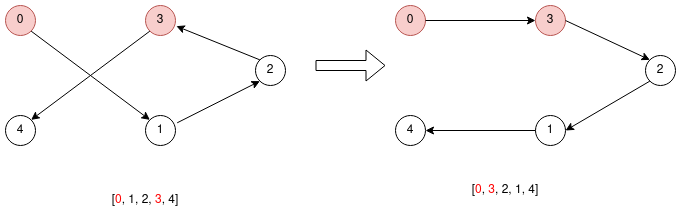
\includegraphics[width=\textwidth]{chapters/literature/img/2exdrawio.png}
      \caption{Przykład procedury 2-exchange}
      \label{fig:2exchange}
\end{figure}
